% SC1004 Chapter 7: Determinants (0->100 ground-up)
\chapter{Determinants}
\label{ch:determinants}

\begin{quote}
\emph{``The determinant is the signed volume of the box the matrix builds.''} Zero means the box is flat --- the matrix squashes space and cannot be undone.
\end{quote}

\noindent\fbox{\parbox{\dimexpr\linewidth-2\fboxsep-2\fboxrule}{%
\textbf{From zero: area before algebra.} We start with area of a parallelogram in $\mathbb{R}^2$ ($ad-bc$), grow to volume in $\mathbb{R}^3$, then axiomatise to $n\times n$ via row operations. Every property is first a picture.}}
\vspace{0.4em}

\section*{Learning Outcomes}
After this chapter you will be able to:
\begin{enumerate}[label=(L\arabic*)]
    \item compute $2\times2$ and $3\times3$ determinants and interpret them as area/volume;
    \item apply row-operation rules and multiplicativity $\det(AB)=\det A\det B$;
    \item use $\det A\neq0$ to test invertibility and find $\det(A^{-1})$;
    \item expand by cofactors and relate to the adjugate;
    \item connect $\det$ to eigenvalues and to Cramer's rule.
\end{enumerate}

% ============================================================
\section{Area, Volume, and the \texorpdfstring{$2\times2$}{2x2} Determinant}
\label{sec:det2x2}
Take columns $\mathbf{a}_1,\mathbf{a}_2\in\mathbb{R}^2$ as edges from the origin. They span a parallelogram. Its signed area is
\[
  \det\begin{bmatrix}a&b\\c&d\end{bmatrix}=ad-bc.
\]
Sign encodes orientation: $\det>0$ means $\mathbf{a}_2$ is counter-clockwise from $\mathbf{a}_1$.

\begin{figure}[h]
\centering
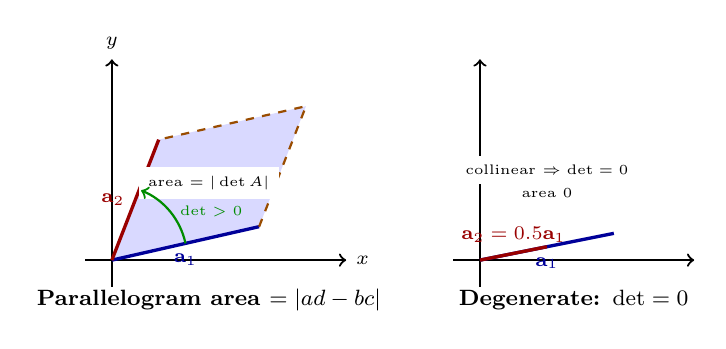
\begin{tikzpicture}[scale=0.85,every node/.style={font=\scriptsize}]
  \draw[->,thick] (-0.4,0)--(3.5,0) node[right] {$x$};
  \draw[->,thick] (0,-0.4)--(0,3.0) node[above] {$y$};
  \fill[blue!15] (0,0)--(2.2,0.5)--(2.9,2.3)--(0.7,1.8)--cycle;
  \draw[very thick,blue!60!black] (0,0)--(2.2,0.5) node[midway,below] {$\mathbf{a}_1$};
  \draw[very thick,red!60!black] (0,0)--(0.7,1.8) node[midway,left] {$\mathbf{a}_2$};
  \draw[thick,orange!60!black,dashed] (2.2,0.5)--(2.9,2.3)--(0.7,1.8);
  \node[font=\tiny,fill=white] at (1.45,1.15) {area $=|\det A|$};
  \draw[->,thick,green!55!black] (1.1,0.25) arc (12:68:1.1) node[midway,right,font=\tiny] {$\det>0$};
  \node[font=\footnotesize\bfseries] at (1.45,-0.6) {Parallelogram area $=|ad-bc|$};

  \begin{scope}[xshift=5.5cm]
    \draw[->,thick] (-0.4,0)--(3.2,0); \draw[->,thick] (0,-0.4)--(0,3.0);
    \fill[red!15] (0,0)--(2.0,0.4)--(2.0,0.4)--cycle;
    \draw[very thick,blue!60!black] (0,0)--(2.0,0.4) node[midway,below] {$\mathbf{a}_1$};
    \draw[very thick,red!60!black] (0,0)--(1.0,0.2) node[midway,above] {$\mathbf{a}_2=0.5\mathbf{a}_1$};
    \node[font=\tiny,fill=white] at (1.0,1.0) {area $0$};
    \node[font=\tiny,fill=white] at (1.0,1.35) {collinear $\Rightarrow\det=0$};
    \node[font=\footnotesize\bfseries] at (1.4,-0.6) {Degenerate: $\det=0$};
  \end{scope}
\end{tikzpicture}
\caption{Left: $\det A$ is the signed area of the column parallelogram. Right: dependent columns give zero area --- the box is flat.}
\label{fig:det-area}
\end{figure}

In $\mathbb{R}^3$, $\det[\mathbf{a}_1\ \mathbf{a}_2\ \mathbf{a}_3]$ is the signed volume of the parallelepiped. The pattern: determinant measures how the matrix scales volumes.

\section{Axioms and Row-Operation Rules}
\label{sec:det-axioms}
For $n\times n$, $\det$ is the unique function $\mathbb{R}^{n\times n}\to\mathbb{R}$ that is (i) multilinear in rows, (ii) alternating (zero if two rows equal), (iii) $\det I_n=1$. From this:

\begin{figure}[h]
\centering
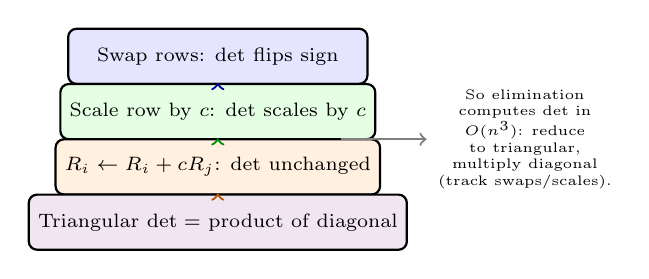
\begin{tikzpicture}[scale=0.78,every node/.style={font=\scriptsize}]
  \node[draw,thick,rounded corners=3pt,fill=blue!10,minimum width=3.8cm,minimum height=0.7cm] (r1) at (0,1.8) {Swap rows: $\det$ flips sign};
  \node[draw,thick,rounded corners=3pt,fill=green!10,minimum width=3.8cm,minimum height=0.7cm] (r2) at (0,0.9) {Scale row by $c$: $\det$ scales by $c$};
  \node[draw,thick,rounded corners=3pt,fill=orange!12,minimum width=3.8cm,minimum height=0.7cm] (r3) at (0,0.0) {$R_i\gets R_i+cR_j$: $\det$ unchanged};
  \node[draw,thick,rounded corners=3pt,fill=violet!10,minimum width=4.2cm,minimum height=0.7cm] (r4) at (0,-0.9) {Triangular $\det=$ product of diagonal};
  \draw[->,thick,blue!60!black] (r1)--(r2);
  \draw[->,thick,green!55!black] (r2)--(r3);
  \draw[->,thick,orange!70!black] (r3)--(r4);
  \node[font=\tiny,align=center] at (5.0,0.45) {So elimination\\computes $\det$ in\\$O(n^3)$: reduce\\to triangular,\\multiply diagonal\\(track swaps/scales).};
  \draw[->,thick,gray] (2.0,0.45)--(3.4,0.45);
\end{tikzpicture}
\caption{How row operations affect the determinant. Elimination to triangular form is the practical algorithm.}
\label{fig:det-rowops}
\end{figure}

Consequences:
\begin{itemize}
    \item $\det(AB)=\det A\cdot\det B$, $\det(A^T)=\det A$.
    \item $A$ invertible $\iff\det A\neq0$, and $\det(A^{-1})=1/\det A$.
    \item $\det(cA)=c^n\det A$ for $n\times n$ (each of $n$ rows scaled).
    \item Row operations as above; column operations obey the same rules ($\det A^T=\det A$).
\end{itemize}

\begin{example}[Via elimination]
$A=\begin{bmatrix}2&1&0\\0&3&1\\1&0&2\end{bmatrix}$. Swap $R_1\leftrightarrow R_3$ flips sign: $\det A=-\det\begin{bmatrix}1&0&2\\0&3&1\\2&1&0\end{bmatrix}$. Then $R_3\gets R_3-2R_1$: $-\det\begin{bmatrix}1&0&2\\0&3&1\\0&1&-4\end{bmatrix}=-1\cdot\det\begin{bmatrix}3&1\\1&-4\end{bmatrix}=-1\cdot(-13)=13$.
\end{example}

\section{Cofactor Expansion and Adjugate}
\label{sec:cofactor}
Delete row $i$, column $j$ from $A$ to get $M_{ij}$ ($n-1\times n-1$). The \emph{cofactor} is $C_{ij}=(-1)^{i+j}\det M_{ij}$. Then for any fixed $i$,
\[
  \det A=\sum_{j=1}^{n} a_{ij}C_{ij}\quad\text{(row $i$ expansion)},
\]
and similarly for any column. The \emph{adjugate} $\operatorname{adj}(A)=[C_{ji}]$ satisfies
\[
  A\cdot\operatorname{adj}(A)=\det(A)\,I_n,
\]
so if $\det A\neq0$, $A^{-1}=\operatorname{adj}(A)/\det A$. For $2\times2$, this is $\frac1{ad-bc}\begin{bmatrix}d&-b\\-c&a\end{bmatrix}$.

Cofactor expansion is $O(n!)$ --- never used for large $n$; elimination is $O(n^3)$.

\begin{figure}[h]
\centering
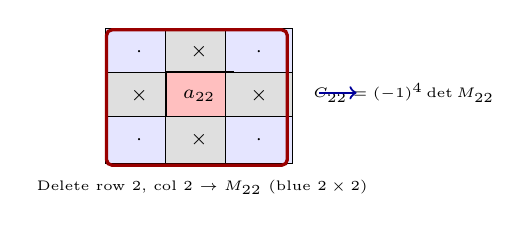
\begin{tikzpicture}[scale=0.80,every node/.style={font=\scriptsize}]
  \foreach \r in {0,...,2} \foreach \c in {0,...,2} {
    \pgfmathparse{(\r==1 && \c==1) ? 1 : 0}
    \ifnum\pgfmathresult=1
      \node[draw,thick,minimum width=0.85cm,minimum height=0.60cm,fill=red!25] at (\c*0.95,\r*-0.70) {$a_{22}$};
    \else
      \pgfmathparse{(\r==1 || \c==1) ? 1 : 0}
      \ifnum\pgfmathresult=1
        \node[draw,minimum width=0.85cm,minimum height=0.60cm,fill=gray!25] at (\c*0.95,\r*-0.70) {$\times$};
      \else
        \node[draw,minimum width=0.85cm,minimum height=0.60cm,fill=blue!10] at (\c*0.95,\r*-0.70) {$\cdot$};
      \fi
    \fi
  }
  \draw[very thick,red!60!black,rounded corners=2pt] (-0.52,0.35)--(2.35,0.35)--(2.35,-1.80)--(-0.52,-1.80)--cycle;
  \node[font=\tiny,fill=white] at (1.0,-2.15) {Delete row 2, col 2 $\to M_{22}$ (blue $2\times2$)};
  \node[font=\tiny,fill=white] at (4.2, -0.65) {$C_{22}=(-1)^{4}\det M_{22}$};
  \draw[->,thick,blue!60!black] (2.85,-0.65)--(3.45,-0.65);
\end{tikzpicture}
\caption{Cofactor $C_{ij}$: delete row $i$ and column $j$, take the determinant of the remaining $(n-1)\times(n-1)$ minor, multiply by $(-1)^{i+j}$.}
\label{fig:cofactor}
\end{figure}

\section{Determinant and Eigenvalues}
\label{sec:det-eigen-preview}
If $A\mathbf{v}=\lambda\mathbf{v}$, then $\det(A-\lambda I)=0$ (Ch.~8). Hence $\det A=\prod_i\lambda_i$ (product of eigenvalues) and $\operatorname{tr}A=\sum_i\lambda_i$. Cramer's rule $x_j=\det A_j/\det A$ (replace column $j$ of $A$ by $\mathbf{b}$) follows from the adjugate but is $O(n!)$ --- a theoretical tool, not an algorithm.

\begin{example}[Python --- determinants]
\begin{lstlisting}[language=Python]
import numpy as np
A = np.array([[2.,1.,0.],[0.,3.,1.],[1.,0.,2.]])
print(np.linalg.det(A))          # ~13.0
print(np.linalg.det(A.T))        # same
print(np.linalg.det(A @ A))      # det(A)^2
# Volume scaling: unit cube -> parallelepiped of volume |det A|
print(abs(np.linalg.det(A)))
\end{lstlisting}
\end{example}

% ============================================================

% --- Additional depth: Properties, geometry in n-dim, and volume scaling ---
\section{Multiplicativity and Invertibility Revisited}
\label{sec:mult-inv}
$\det(AB)=\det A\det B$ implies $\det(A^{-1})=1/\det A$ and $\det(PAP^{-1})=\det A$ (similarity preserves $\det$). Hence $\det$ is a basis-free invariant of the linear map $T:\mathbf{x}\mapsto A\mathbf{x}$: it is the volume scaling factor of $T$, independent of coordinates.

\begin{theorem}[Volume scaling]
For any measurable $S\subset\mathbb{R}^n$, $\operatorname{vol}(A(S))=|\det A|\cdot\operatorname{vol}(S)$ when $A$ is invertible. $|\det A|$ is the factor by which $A$ stretches $n$-dimensional volume; $\det A=0$ collapses volume to zero.
\end{theorem}
This is why $|\det J|$ appears as the Jacobian in change of variables for integrals.

\section{Determinant, Rank, and Eigenvalues}
\label{sec:det-rank-eigen}
$\det A\neq0\iff\operatorname{rank}A=n\iff0$ is not an eigenvalue. More generally, $\det A=\prod_{i=1}^n\lambda_i$ where $\lambda_i$ are eigenvalues (with algebraic multiplicity, possibly complex). So $|\det A|$ is the product of singular values too (Ch.~8 notes). For triangular $A$, $\det$ is the diagonal product --- eigenvalues sit on the diagonal.

\begin{example}[When $\det$ misleads]
$A=0.1\,I_{100}$ has $\det A=10^{-100}$ (tiny) but $A$ is perfectly invertible ($\kappa=1$). Determinant magnitude does not measure near-singularity; condition number does. Never test ``$\det\approx0$'' for invertibility in floating point.
\end{example}

\section{Cramer's Rule and Its Cost}
\label{sec:cramer-detail}
If $A$ invertible, $A^{-1}=\operatorname{adj}(A)/\det A$ and $x_j=\det A_j/\det A$ where $A_j$ replaces column $j$ by $\mathbf{b}$. Cost $O(n!)$ via cofactors vs.\ $O(n^3)$ via $LU$: for $n=20$, $20!\approx2.4\times10^{18}$ --- intractable. Cramer is a theoretical gem that proves $A^{-1}$ entries are rational functions of $A$'s entries.



\begin{remark}[Orientation and handedness]
In graphics, $\det>0$ means a right-handed coordinate frame stays right-handed after $A$; $\det<0$ means it flips (mirror). This is why $\det$ of a rotation is $+1$ and of a reflection is $-1$ --- the sign is the parity of the transformation.
\end{remark}

\begin{example}[Determinant and invertibility in code]
Never branch on \texttt{det(A)==0} in floating point; use \texttt{np.linalg.matrix\_rank} or \texttt{cond}. For $n=100$, round-off makes $\det$ under/overflow ($\sim10^{\pm100}$) while rank via SVD is reliable. Check \texttt{np.linalg.cond(A)} --- large means near-singular regardless of $\det$ scale.
\end{example}



\begin{example}[Triangular shortcut]
If $U$ is upper-triangular, $\det U=\prod u_{ii}$ immediately. So in $PA=LU$, $\det A=\pm\prod u_{ii}$ (sign $=$ parity of row swaps in $P$). This is the $O(n^3)$ algorithm; no cofactor needed. For $2\times2$, both routes agree: $\det\begin{bmatrix}a&b\\c&d\end{bmatrix}=ad-bc$.
\end{example}


\section{Chapter Notes}
Cauchy and Jacobi formalised $\det(AB)=\det A\det B$; Laplace gave the expansion. Modern libraries compute $\det$ via $LU$ with partial pivoting and track sign; for large $n$, $\log|\det|$ is returned to avoid overflow. The volume picture generalises to $|\det|$ as the Jacobian in multivariate calculus.

% ============================================================
\section{Exercises}
\label{sec:ch07-exercises}
\begin{enumerate}[label=E7.\arabic*, leftmargin=*, itemsep=0.8em]
\item \textbf{Compute.} Find $\det A$ for $A=\begin{bmatrix}3&1&2\\0&-1&4\\1&0&1\end{bmatrix}$ by (a) row operations to triangular and (b) cofactor expansion along row 2. Compare.
\item \textbf{Invertibility.} For which $c$ is $A=\begin{bmatrix}1&c&0\\c&1&0\\0&0&2\end{bmatrix}$ singular? Relate to volume collapse and to eigenvalues.
\item \textbf{Rules.} Prove $\det(cA)=c^n\det A$ for $n\times n$ using the multilinear axiom. Use $\det(AB)=\det A\det B$ to show $\det(A^{-1})=1/\det A$ when invertible.
\item \textbf{Cramer.} Solve $\begin{cases}x+2y=5\\3x-y=1\end{cases}$ via Cramer's rule and compare with elimination. Why is Cramer $O(n!)$ and not used for $n>3$?
\item \textbf{Coding.} For random $n\times n$ matrices ($n=10,50,100$), compare \texttt{np.linalg.det} (via $LU$) with a cofactor implementation for $n\le6$ (time and overflow). Plot $\log|\det|$ vs.\ $n$.
\end{enumerate}
% End of Chapter 7
